\subsection{Artificial Neural Network (ANN -- MLP)}\label{subsec:ann}

\subsubsection{Cơ sở lý thuyết}

\paragraph{1. Kiến trúc mạng truyền thẳng nhiều tầng (Multi-Layer Perceptron)}\mbox{}\\
Xét tập dữ liệu huấn luyện gồm $N$ mẫu $\{(\mathbf{x}_n, y_n)\}_{n=1}^{N}$, trong đó $\mathbf{x}_n \in \mathbb{R}^D$ là vector đặc trưng đầu vào và nhãn nhị phân $y_n \in \{0, 1\}$ đại diện lần lượt cho hai lớp $\mathcal{C}_0$ (bình thường) và $\mathcal{C}_1$ (gian lận). Mạng nơ-ron nhân tạo truyền thẳng nhiều tầng (\textit{Multi-Layer Perceptron -- MLP}) là mô hình học có giám sát có khả năng xấp xỉ các ánh xạ phi tuyến phức tạp thông qua $L$ tầng kết nối đầy đủ (\textit{fully-connected layers}), bao gồm tầng đầu vào ($\mathbf{a}^{(0)} = \mathbf{x}$), các tầng ẩn ($l = 1, \dots, L - 1$) và tầng đầu ra ($l = L$).

Tại mỗi tầng $l \in \{1, \dots, L\}$, quá trình lan truyền xuôi (\textit{forward propagation}) thực hiện phép biến đổi tuyến tính theo sau bởi hàm kích hoạt phi tuyến $g^{(l)}(\cdot)$:
\begin{equation}
    \mathbf{z}^{(l)} = \mathbf{W}^{(l)} \mathbf{a}^{(l-1)} + \mathbf{b}^{(l)}, \qquad \mathbf{a}^{(l)} = g^{(l)}\big(\mathbf{z}^{(l)}\big)
\end{equation}
trong đó $\mathbf{W}^{(l)} \in \mathbb{R}^{d_l \times d_{l-1}}$ là ma trận trọng số kết nối giữa tầng $l - 1$ và tầng $l$, $\mathbf{b}^{(l)} \in \mathbb{R}^{d_l}$ là vector độ lệch (\textit{bias}), và $d_l$ là số nơ-ron tại tầng $l$. Kiến trúc mạng MLP với hai tầng ẩn được minh họa tại Hình~\ref{fig:ann-architecture}.

\begin{figure}[H]
    \centering
    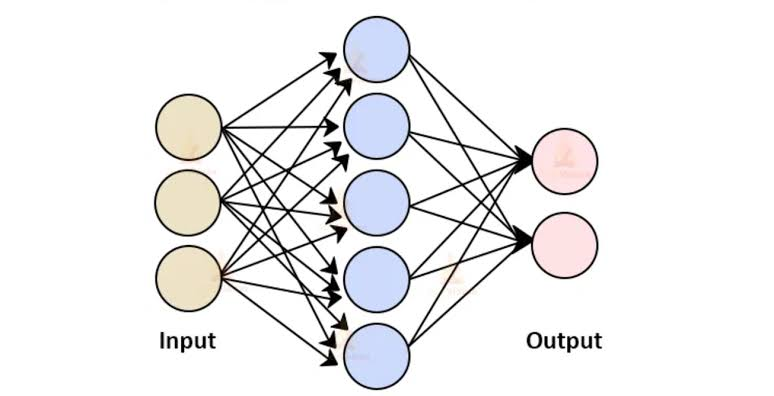
\includegraphics[width=0.75\linewidth]{graphics/ann_architecture.jpg}
    \caption{Minh họa kiến trúc mạng nơ-ron truyền thẳng nhiều tầng (MLP) với hai tầng ẩn}
    \label{fig:ann-architecture}
\end{figure}

\paragraph{2. Hàm kích hoạt phi tuyến (ReLU và Sigmoid)}\mbox{}\\
Nhằm tránh việc hợp thành nhiều tầng tuyến tính suy biến thành một ánh xạ tuyến tính duy nhất, các tầng ẩn sử dụng hàm kích hoạt \textbf{ReLU} (\textit{Rectified Linear Unit}):
\begin{equation}
    g_{\text{ReLU}}(z) = \max(0, z), \qquad g'_{\text{ReLU}}(z) = \begin{cases}
        1 & \text{nếu } z > 0 \\
        0 & \text{nếu } z \le 0
    \end{cases}
\end{equation}
Hàm ReLU giúp tính toán nhanh, tạo biểu diễn thưa cho các nơ-ron ẩn và giảm đáng kể hiện tượng triệt tiêu đạo hàm (\textit{vanishing gradient}) trên miền dương so với Sigmoid hoặc Tanh (Hình~\ref{fig:ann-relu}).

\begin{figure}[H]
    \centering
    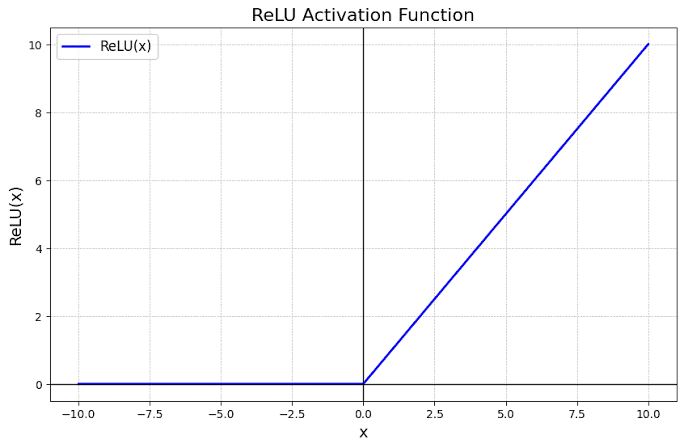
\includegraphics[width=0.65\linewidth]{graphics/ann_relu.png}
    \caption{Đồ thị hàm kích hoạt ReLU $g(z) = \max(0, z)$ và đạo hàm $g'(z)$}
    \label{fig:ann-relu}
\end{figure}

Tại tầng đầu ra ($l = L$, $d_L = 1$), đầu ra tuyến tính $z^{(L)}$ đi qua hàm kích hoạt \textbf{Sigmoid} để ước lượng xác suất hậu nghiệm thuộc lớp gian lận $\mathcal{C}_1$:
\begin{equation}
    \hat{y} \triangleq p(\mathcal{C}_1 \mid \mathbf{x}, \Theta) = \sigma\big(z^{(L)}\big) = \frac{1}{1 + e^{-z^{(L)}}} \in (0, 1)
\end{equation}
với $\Theta = \{(\mathbf{W}^{(l)}, \mathbf{b}^{(l)})\}_{l=1}^{L}$ là tập toàn bộ tham số cần học. Nhãn dự đoán $\hat{t} \in \{0, 1\}$ được xác định theo ngưỡng quyết định $\lambda$ (mặc định $\lambda = 0.5$): $\hat{t} = 1$ nếu $\hat{y} \ge \lambda$ và $\hat{t} = 0$ nếu ngược lại.

\paragraph{3. Hàm mất mát, Lan truyền ngược và Bộ tối ưu Adam}\mbox{}\\
Để huấn luyện mô hình phân loại nhị phân đồng thời kiểm soát độ phức tạp trọng số chống quá khớp (\textit{overfitting}), hàm mục tiêu sử dụng \textbf{Binary Cross-Entropy} kết hợp thành phần điều chuẩn \textbf{L2} (\textit{weight decay}):
\begin{equation}
    \mathcal{J}(\Theta) = -\frac{1}{N} \sum_{n=1}^{N} \left[ y_n \log \hat{y}_n + (1 - y_n) \log(1 - \hat{y}_n) \right] + \frac{\alpha}{2N} \sum_{l=1}^{L} \|\mathbf{W}^{(l)}\|_F^2
\end{equation}
trong đó $\alpha > 0$ là hệ số điều chuẩn L2 và $\|\cdot\|_F$ là chuẩn Frobenius của ma trận trọng số.

Gradient của hàm mục tiêu $\mathbf{g}_t = \nabla_{\Theta}\mathcal{J}(\Theta_{t-1})$ trên từng \textit{mini-batch} được tính hiệu quả bằng thuật toán \textbf{lan truyền ngược (Backpropagation)} dựa trên quy tắc dây chuyền (\textit{chain rule}). Quá trình cập nhật tham số sử dụng bộ tối ưu \textbf{Adam} (\textit{Adaptive Moment Estimation}), kết hợp ước lượng trung bình trượt hàm mũ của gradient bậc nhất ($\mathbf{m}_t$) và bình phương gradient bậc hai ($\mathbf{v}_t$):
\begin{equation}
    \mathbf{m}_t = \beta_1 \mathbf{m}_{t-1} + (1 - \beta_1)\mathbf{g}_t, \qquad \mathbf{v}_t = \beta_2 \mathbf{v}_{t-1} + (1 - \beta_2)\mathbf{g}_t^2
\end{equation}
Sau khi hiệu chỉnh độ chệch khởi tạo $\hat{\mathbf{m}}_t = \frac{\mathbf{m}_t}{1 - \beta_1^t}$ và $\hat{\mathbf{v}}_t = \frac{\mathbf{v}_t}{1 - \beta_2^t}$, tham số mạng được cập nhật theo công thức:
\begin{equation}
    \Theta_t = \Theta_{t-1} - \eta \frac{\hat{\mathbf{m}}_t}{\sqrt{\hat{\mathbf{v}}_t} + \epsilon}
\end{equation}
trong đó $\eta$ là tốc độ học ban đầu, $\beta_1, \beta_2 \in [0, 1)$ là các hệ số suy giảm mô-men và $\epsilon > 0$ giúp ổn định số học khi chia. Nhờ cơ chế tự điều chỉnh tốc độ học riêng cho từng tham số, Adam hội tụ nhanh và ổn định trên dữ liệu quy mô lớn.

\subsubsection{Áp dụng mô hình vào bài toán}

\paragraph{1. Môi trường và Thư viện sử dụng}\mbox{}\\
Mô hình được cài đặt bằng ngôn ngữ \textbf{Python} với hai thư viện chính:
\begin{itemize}
    \item \texttt{scikit-learn}: Cung cấp lớp \texttt{MLPClassifier} để xây dựng và huấn luyện mạng nơ-ron nhiều tầng, cùng \texttt{RobustScaler} và \texttt{StratifiedKFold} cho bước chuẩn hóa và kiểm định chéo.
    \item \texttt{NumPy}: Hỗ trợ xử lý mảng và tính toán vector hóa dữ liệu.
\end{itemize}

\paragraph{2. Quy trình tiền xử lý và Huấn luyện}\mbox{}\\
Quy trình thực nghiệm trong tệp \texttt{src/model\_ANN.py} tuân thủ chặt chẽ nguyên tắc cô lập tập kiểm định để tránh rò rỉ dữ liệu (\textit{data leakage}):
\begin{enumerate}
    \item \textbf{Phân chia dữ liệu phân tầng:} Tập dữ liệu sau làm sạch được tách thành tập huấn luyện toàn phần và tập kiểm tra độc lập (\texttt{split\_train\_test}), kết hợp kiểm định chéo \textit{Stratified K-Fold} nhằm giữ nguyên tỷ lệ lớp gian lận trên từng \textit{fold}.
    \item \textbf{Chuẩn hóa đặc trưng kháng ngoại lai:} Do mạng nơ-ron tối ưu theo gradient nên rất nhạy với độ lớn đầu vào. Trong khi các thành phần \texttt{V1--V28} đã qua biến đổi PCA, cột đặc trưng giao dịch (\texttt{COLS\_TO\_SCALE}) được chuẩn hóa bằng \texttt{RobustScaler} (chỉ \texttt{fit\_transform} trên tập huấn luyện con rồi \texttt{transform} sang tập kiểm định).
    \item \textbf{Huấn luyện có dừng sớm và Đánh giá:} Trong từng \textit{fold}, mô hình \texttt{MLPClassifier} được huấn luyện với cơ chế \texttt{early\_stopping=True} (tự động trích $10\%$ tập huấn luyện làm tập kiểm định nội bộ để dừng sớm khi hiệu năng không cải thiện, vừa hạn chế quá khớp vừa rút ngắn thời gian chạy). Sau khi hoàn tất kiểm định chéo, mô hình cuối cùng được huấn luyện lại trên toàn bộ tập huấn luyện đã chuẩn hóa và đánh giá trên tập kiểm tra với ngưỡng phân loại $\lambda = 0.5$ qua mô-đun \texttt{src/metrics.py}.
\end{enumerate}

\paragraph{3. Thiết lập siêu tham số}\mbox{}\\
Cấu hình chi tiết trong hàm \texttt{build\_model()} của tệp \texttt{src/model\_ANN.py} được tổng hợp tại Bảng~\ref{tab:ann_hyperparams}.

\begin{table}[H]
\centering
\caption{Thiết lập siêu tham số cho mô hình Artificial Neural Network (\texttt{src/model\_ANN.py})}
\label{tab:ann_hyperparams}
\renewcommand{\arraystretch}{1.2}
\begin{tabular}{|l|l|p{8.0cm}|}
\hline
\textbf{Siêu tham số} & \textbf{Giá trị} & \textbf{Mục đích sử dụng} \\
\hline
\texttt{hidden\_layer\_sizes} & \texttt{(64, 32)} & Thiết kế 2 tầng ẩn với 64 và 32 nơ-ron, đủ khả năng biểu diễn quan hệ phi tuyến mà vẫn gọn nhẹ, tránh quá khớp. \\
\hline
\texttt{activation} & \texttt{"relu"} & Hàm kích hoạt ReLU cho các tầng ẩn, tăng tốc độ tính toán và hạn chế triệt tiêu gradient. \\
\hline
\texttt{solver} & \texttt{"adam"} & Bộ tối ưu hóa Adam thích ứng tốc độ học theo từng tham số, hội tụ nhanh trên dữ liệu lớn. \\
\hline
\texttt{max\_iter} & \texttt{50} & Giới hạn tối đa 50 vòng lặp (\textit{epochs}) giúp kiểm soát thời gian huấn luyện trên toàn bộ 5 \textit{folds}. \\
\hline
\texttt{early\_stopping} & \texttt{True} & Tự động dừng sớm dựa trên tập kiểm định nội bộ ($10\%$) khi điểm số không còn cải thiện, hạn chế quá khớp. \\
\hline
\texttt{random\_state} & \texttt{42} & Cố định hạt giống khởi tạo trọng số ngẫu nhiên và chia lô nhằm đảm bảo tính tái lập kết quả. \\
\hline
\end{tabular}
\end{table}
